\documentclass[11pt]{article}

\usepackage[margin=1in]{geometry}
\usepackage[T1]{fontenc}
\usepackage{lmodern}
\usepackage{microtype}
\usepackage{amsmath,amssymb,amsfonts}
\usepackage{booktabs}
\usepackage{longtable}
\usepackage{array}
\usepackage{enumitem}
\usepackage{graphicx}
\usepackage{xcolor}
\usepackage{hyperref}
\usepackage{natbib}

\hypersetup{
  colorlinks=true,
  linkcolor=blue!55!black,
  citecolor=blue!55!black,
  urlcolor=blue!55!black
}

\setlist[itemize]{leftmargin=1.6em}
\setlist[enumerate]{leftmargin=1.8em}
\newcommand{\code}[1]{\texttt{#1}}
\newcommand{\ellij}{\ell_{ij}}
\newcommand{\R}{\mathbb{R}}
\newcommand{\E}{\mathcal{E}}
\newcommand{\diag}{\operatorname{diag}}
\newcommand{\tr}{\operatorname{tr}}
\newcommand{\vol}{\operatorname{vol}}
\newcommand{\argmin}{\operatorname*{arg\,min}}

\title{Conductance and Kernel Choices for Graph Laplacians:\\
Theory, Tasks, and Implications for Graph Low-Pass Smoothing}
\author{SIMODS Provenance/Librarian synthesis from H005 reviewer-auditor memos}
\date{Built 2026-05-15 09:00:10 EDT}

\begin{document}
\maketitle

\begin{abstract}
This report synthesizes ten full-paper reviews and audits on graph conductance
and kernel choices for Laplacians, diffusion operators, semi-supervised graph
regression, manifold learning, and graph signal smoothing.  The immediate
SIMODS purpose is methodological: to guide a future benchmark that compares the
current \code{gflow} low-pass/GCV smoother with length- and kernel-conductance
alternatives.  The central conclusion is that researchers rarely choose
conductances only as inverse metric lengths.  Gaussian kernels, heat kernels,
self-tuned/local-scale kernels, density-normalized kernels, Markov
normalizations, and graph-spectral filters each encode a different answer to
the question ``what should count as a smooth signal on this graph?''  These
choices change the graph energy, the eigenbasis, the diffusion geometry, and
therefore the behavior of low-pass smoothing and GCV.  For SIMODS, the current
\code{fit.rdgraph.regression()} operator must be kept conceptually separate
from these planned comparators: the current precomputed-graph path uses supplied
edge lengths for local neighborhood ordering/truncation and then constructs an
overlap-density/Riemannian-complex conductance, not direct inverse-length,
Gaussian, or self-tuned conductances.
\end{abstract}

\tableofcontents
\newpage

\section{Review Corpus and Evidence Conventions}

This synthesis is based on the H005 review workspace
\code{literature/conductance\_kernel\_laplacian\_review}.  The source manifest
records the canonical reading copy for each Tier 1 paper, including original
URL, DOI or arXiv identifier when available, local path, access date, page
count, and SHA-256.  Each Tier 1 paper was assigned to a dedicated reviewer and
a dedicated auditor.  Reviewers read the whole paper, including figures.
Auditors checked formulas, operator definitions, figure references, evidence
labels, and relevance to \code{gflow}/SIMODS.  All ten audits returned minor
revisions; no auditor requested a full reread.  The review memos now include
post-audit revision notes.

The evidence labels used here are:

\begin{description}
  \item[explicit] The claim is directly stated in the reviewed paper.
  \item[derived] The claim follows from formulas, algorithms, figures, or
    experiments in the paper, but is not stated in exactly this language.
  \item[contextual] The claim is our SIMODS/gflow interpretation or
    cross-paper synthesis.
  \item[uncertain] The claim is plausible but ambiguous, typographically
    suspect, or awaiting developer/paper confirmation.
\end{description}

Unless otherwise marked, paper-specific statements in the paper-by-paper
section are summaries of explicit or directly derived review findings.  The
SIMODS recommendations are contextual.

\begin{longtable}{p{0.08\linewidth}p{0.40\linewidth}p{0.20\linewidth}p{0.22\linewidth}}
\caption{Tier 1 corpus and review role in the synthesis.}\\
\toprule
ID & Paper & Main conductance/kernel theme & Main SIMODS role\\
\midrule
\endhead
P01 & \citet{zelnikmanor2004selftuning} & self-tuned local-scale Gaussian affinity & adaptive/local-scale comparator\\
P02 & \citet{belkin2001laplacian} & heat-kernel and binary graph weights for Laplacian Eigenmaps & heat-kernel manifold-learning baseline\\
P03 & \citet{coifman2006diffusion} & kernel, density normalization, Markov diffusion & diffusion/Markov normalization baseline\\
P04 & \citet{berry2016variable} & variable-bandwidth diffusion kernels & local-bandwidth and density-correction theory\\
P05 & \citet{zhu2003semisupervised} & graph weights for harmonic-function semi-supervised learning & graph interpolation/regression analogue\\
P06 & \citet{belkin2006manifold} & graph Laplacian regularization in learning & regularization objective analogue\\
P07 & \citet{shuman2013emerging} & graph Fourier bases and spectral filters & graph low-pass smoothing semantics\\
P08 & \citet{hein2007graph} & convergence of graph Laplacians on random neighborhood graphs & normalization and density-limit warnings\\
P09 & \citet{belkin2008towards} & theoretical foundation for Laplacian manifold methods & heat-kernel/Laplace-Beltrami theory baseline\\
P10 & \citet{cheng2022knn} & kNN self-tuned kernel graph Laplacian convergence & adaptive/kNN local-scale theory\\
\bottomrule
\end{longtable}

\section{Primer: From Lengths to Conductances to Smoothers}

\subsection{Weighted Graph Laplacians}

Let \(G=(V,E)\) be an undirected graph with \(n=|V|\) vertices.  A graph signal
is a vector \(f\in\R^n\), or a matrix \(F\in\R^{n\times p}\) when \(p\)
features are smoothed on the same graph.  A nonnegative edge weight
\[
  c_{ij}=c_{ji}\ge 0
\]
can be called an affinity, similarity, weight, or conductance depending on the
paper and task.  With weighted adjacency \(W=(c_{ij})\), degree
\(D_{ii}=\sum_j c_{ij}\), and unnormalized Laplacian \(L=D-W\), the standard
Dirichlet energy is
\[
  \E_G(f)
  =
  f^\top L f
  =
  \frac12\sum_{i,j} c_{ij}(f_i-f_j)^2
  =
  \sum_{\{i,j\}\in E} c_{ij}(f_i-f_j)^2.
\]
The factor convention matters.  Several reviewed papers print unhalved double
sums while also writing \(f^\top Lf\).  This does not change minimizers, but it
does matter for precise comparisons of objectives and constants.

For a matrix signal \(F\), the analogous energy is
\[
  \tr(F^\top L F)
  =
  \frac12\sum_{i,j} c_{ij}\|F_i-F_j\|^2.
\]
Large \(c_{ij}\) makes disagreement across edge \((i,j)\) expensive.  Thus the
conductance rule determines what functions are low energy before any smoothing
parameter is chosen.

\subsection{A Common Family of Conductance Rules}

The review treats many formulas as members of a common family
\[
  c_{ij}=\phi(\ell_{ij};\theta),
\]
where \(\ell_{ij}\) is an ambient distance, graph edge length, or local
dissimilarity, and \(\theta\) includes bandwidth, exponent, local bandwidth,
density, or normalization parameters.  Important examples are:
\begin{align}
  c_{ij}^{\mathrm{len}} &= (\ell_{ij}+\epsilon)^{-\alpha},\\
  c_{ij}^{\mathrm{exp}} &= \exp(-\ell_{ij}/\sigma),\\
  c_{ij}^{\mathrm{rbf}} &= \exp(-\ell_{ij}^2/\sigma^2),\\
  c_{ij}^{\mathrm{self}} &= \exp\!\left(-\frac{\ell_{ij}^2}{\sigma_i\sigma_j}\right),\\
  c_{ij}^{\mathrm{vb}} &=
    h\!\left(\frac{\ell_{ij}^2}{\epsilon \rho_i\rho_j}\right).
\end{align}
The inverse-length rule is natural when edge length is interpreted as physical
resistance or cost.  Heat/RBF kernels are natural when the graph is meant to
approximate local heat diffusion on a point cloud or manifold.  Self-tuned and
variable-bandwidth kernels are natural when a single global scale fails under
nonuniform sampling.  Density-normalized kernels are natural when the target is
geometry rather than sampling density.

\subsection{Low-Pass Filtering}

If \(L=V\Lambda V^\top\) is a symmetric graph Laplacian eigendecomposition, a
spectral graph filter has the form
\[
  S_h = Vh(\Lambda)V^\top,
\]
where \(h(\lambda)\) attenuates high-frequency modes.  Heat smoothing uses
\(h_t(\lambda)=\exp(-t\lambda)\).  Tikhonov smoothing uses
\[
  h_\eta(\lambda)=\frac{1}{1+\eta\lambda}
\]
or an equivalent parameterization.  More general graph signal processing
filters may be polynomial, idealized low-pass, Butterworth-like, or learned,
but they all inherit their meaning from the graph eigenbasis.

If the operator is a row-stochastic diffusion matrix \(P\) with eigenvalues
\(\lambda_j\), diffusion powers use \(h_t(\lambda_j)=\lambda_j^t\).  This is
low-pass relative to the Markov operator: slowly varying modes have eigenvalues
near 1 and survive many diffusion steps.

\subsection{Current gflow Smoother Versus Planned Comparators}

The H003/H004/H005 line of work needs one hard distinction.  The current
\code{fit.rdgraph.regression()} precomputed-graph path does not convert
supplied edge lengths directly into conductances by
\[
  c_e=\frac{1}{\ell_e+\epsilon}.
\]
As established in the companion source audit, supplied \code{weight.list}
values are positive graph edge lengths used for local neighborhood ordering and
truncation.  The mass-symmetrized spectral smoother then uses an
overlap-density/Riemannian-complex edge mass \(\rho_1(e)\), with conductance
\[
  c_e^\rho=\frac{1}{\max(\rho_1(e),10^{-10})}.
\]
Therefore the papers reviewed here mainly support planned comparator families:
inverse-length, heat/RBF, exponential, self-tuned, variable-bandwidth,
density-normalized, and Markov diffusion smoothers.  They do not retroactively
describe the current \code{gflow} smoother.

\section{Concept Map}

The concepts in this review form a pipeline, not a list of interchangeable
phrases:
\[
\begin{array}{ccccc}
\text{edge length } \ell_{ij}
&\longrightarrow&
\text{conductance/affinity } c_{ij}
&\longrightarrow&
\text{operator } L \text{ or } P\\[3pt]
&& \downarrow && \downarrow\\[3pt]
&& \text{graph energy/eigenbasis}
&& \text{filter } h(\lambda) \text{ or diffusion time } t\\[3pt]
&& \multicolumn{3}{c}{\downarrow}\\[3pt]
&& \multicolumn{3}{c}{\text{graph low-pass smoothing and GCV}}
\end{array}
\]

The main branches are:
\begin{itemize}
  \item \textbf{Inverse length conductance} treats short edges as strong
    couplings and long edges as weak couplings.  It is close to physical
    resistance/conductance intuition and directly tests graph metric geometry.
  \item \textbf{Heat kernels} convert squared local distances into local
    diffusion affinities.  They are central in Laplacian Eigenmaps and
    Laplace-Beltrami approximation.
  \item \textbf{Self-tuned/local-scale kernels} replace a global bandwidth with
    endpoint scales such as \(\sigma_i\sigma_j\), reducing global-scale
    fragility under nonuniform sampling.
  \item \textbf{Adaptive-radius/cKNN graph construction} changes the support of
    the graph.  This is related to, but not identical to, self-tuned
    conductance weighting.  A paper may use nearest-neighbor distances for
    bandwidths without defining cKNN support.
  \item \textbf{Diffusion/Markov normalization} changes affinities into a
    random-walk operator \(P\).  The resulting eigenfunctions and smoothing
    behavior depend on degree and density normalization.
  \item \textbf{Graph low-pass smoothing} applies a spectral response
    \(h(\lambda)\) to the operator eigensystem.  P07 is the clearest source for
    this filter semantics.
\end{itemize}

\section{Paper-by-Paper Reviews}

\subsection{P01: Self-Tuning Spectral Clustering}

\citet{zelnikmanor2004selftuning} address a concrete failure mode of spectral
clustering: one global Gaussian bandwidth can be too small for sparse regions
and too large for dense regions.  The paper modifies the Ng-Jordan-Weiss
pipeline by replacing the global Gaussian affinity
\[
  A_{ij}=\exp\left(-\frac{d^2(s_i,s_j)}{\sigma^2}\right)
\]
with the self-tuned affinity
\[
  \hat A_{ij}=
  \exp\left(-\frac{d^2(s_i,s_j)}{\sigma_i\sigma_j}\right),
  \qquad
  \sigma_i=d(s_i,s_K),
\]
where \(s_K\) is the \(K\)th neighbor of \(s_i\).  The normalized affinity
operator is \(L=D^{-1/2}\hat A D^{-1/2}\).  In the paper's terminology,
\(\hat A\) is an affinity; interpreting it as a conductance is our graph
smoothing translation.

The paper's figures make the scale argument vivid.  Figure 1 shows global
bandwidth sensitivity.  Figure 2 shows the central local-scale effect: local
scaling weakens cross-cluster affinities that are misleading under a single
global bandwidth.  Figures 3--6 cover synthetic clustering, eigenvalue-gap
limitations, alignment costs for estimating the number of clusters, and image
segmentation.

\begin{figure}[htbp]
\centering
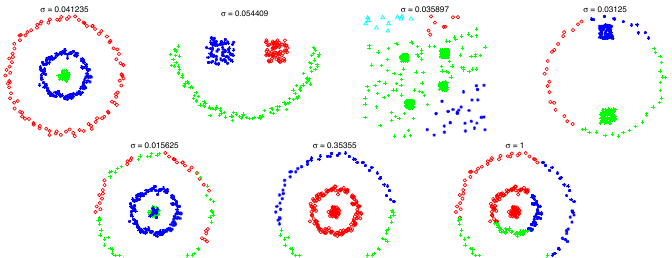
\includegraphics[width=0.31\linewidth]{paper_figures/P01_F01_page02.png}
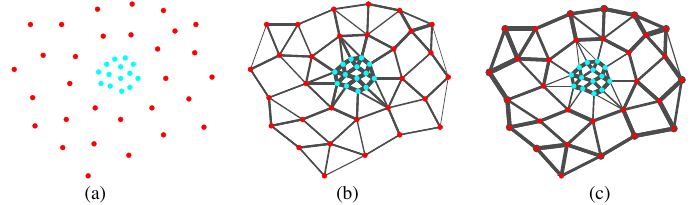
\includegraphics[width=0.31\linewidth]{paper_figures/P01_F02_page03.png}
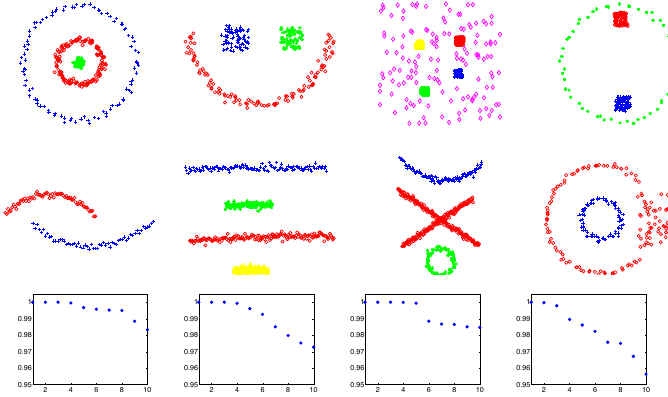
\includegraphics[width=0.31\linewidth]{paper_figures/P01_F03_F04_page04.png}\\[0.5em]
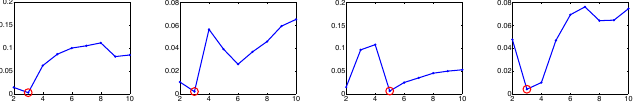
\includegraphics[width=0.31\linewidth]{paper_figures/P01_F05_page06.png}
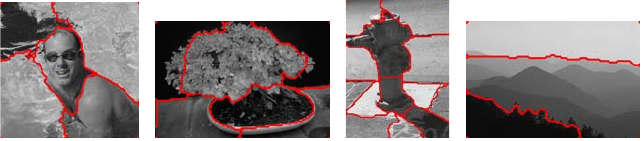
\includegraphics[width=0.31\linewidth]{paper_figures/P01_F06_page07.png}
\caption{Cropped figure panels containing the P01 figures discussed above.
Reproduced from Zelnik-Manor and Perona (2004), Figures 1--6, PDF pp. 2--7,
from the canonical reading copy, for internal review only.}
\end{figure}

For SIMODS, P01 is the prototype for a self-tuned Gaussian comparator.  It does
not define cKNN support or adaptive-radius graph construction.  Its
nearest-neighbor distances set bandwidths, not necessarily graph support.
Thus a SIMODS cKNN connection is contextual synthesis.  The reviewer/auditor
also flagged an ambiguity: Eq. (3) as printed gives an ideal per-row cost of 1,
whereas Figure 5 plots near-zero alignment costs.  The final manuscript should
not rely on the exact plotted cost scale.

\subsection{P02: Laplacian Eigenmaps}

\citet{belkin2001laplacian} give one of the clearest early pipelines from
point-cloud neighborhoods to graph Laplacian eigenvectors.  Build a graph by an
\(\epsilon\)-neighborhood rule or symmetrized nearest-neighbor rule; assign
either heat weights
\[
  W_{ij}=\exp\left(-\frac{\|x_i-x_j\|^2}{t}\right)
\]
or binary weights; solve
\[
  Ly=\lambda Dy,\qquad L=D-W;
\]
and use the first nontrivial eigenvectors as embedding coordinates.

The paper's heat-kernel derivation prints the short-time local heat kernel
\[
  H_t(x,y)\approx (4\pi t)^{-n/2}
  \exp\left(-\frac{\|x-y\|^2}{4t}\right).
\]
Thus the paper contains both \(t\) and \(4t\) bandwidth conventions.  They
should be preserved as printed rather than silently merged.

The core variational identity is
\[
  y^\top Ly=\frac12\sum_{i,j}(y_i-y_j)^2W_{ij}.
\]
For vector-valued embeddings,
\[
  \tr(Y^\top LY)=\frac12\sum_{i,j}\|Y_i-Y_j\|^2W_{ij}.
\]
The paper sometimes writes unhalved objectives; this is an irrelevant
constant for minimizers but should be stated.  P02 is a strong source for heat
weights and graph smoothness, but not for density correction, local bandwidth,
or current \code{gflow} overlap-density smoothing.

\subsection{P03: Diffusion Maps}

\citet{coifman2006diffusion} move from symmetric affinities to Markov diffusion
geometry.  Starting with a symmetric nonnegative kernel \(k(x,y)\), define
\[
  d(x)=\int k(x,y)\,d\mu(y),\qquad
  p(x,y)=\frac{k(x,y)}{d(x)}.
\]
The row-stochastic operator \(P\) has powers \(P^t\), and the diffusion
distance is the distance between \(t\)-step transition distributions.  If
\(P\psi_\ell=\lambda_\ell\psi_\ell\), then
\[
  D_t(x,y)^2=\sum_{\ell\ge 1}\lambda_\ell^{2t}
  \big(\psi_\ell(x)-\psi_\ell(y)\big)^2,
\]
and the diffusion map uses coordinates
\[
  \Psi_t(x)=
  (\lambda_1^t\psi_1(x),\ldots,\lambda_s^t\psi_s(x)).
\]

This paper is crucial because it separates three issues: the kernel, the
degree/Markov normalization, and the diffusion time.  Section 3 introduces
\(\alpha\)-normalization,
\[
  k_\epsilon^{(\alpha)}(x,y)
  =
  \frac{k_\epsilon(x,y)}
       {q_\epsilon(x)^\alpha q_\epsilon(y)^\alpha},
\]
which changes the limiting operator.  In particular, \(\alpha=1\) removes
sampling-density bias in the Laplace-Beltrami limit, while other values retain
density-dependent terms.

For graph low-pass smoothing, P03 gives the Markov counterpart of spectral
filtering: \(P^t\) multiplies mode \(\ell\) by \(\lambda_\ell^t\), damping
small-eigenvalue modes of \(P\).  Calling Figure 3 a graph-signal low-pass
figure is derived synthesis, not the paper's own terminology.  The audit also
flagged the Section 3.4 \(\alpha=0\) phrase as an apparent typo because the
heading and proposition concern \(\alpha=1\).

\begin{figure}[htbp]
\centering
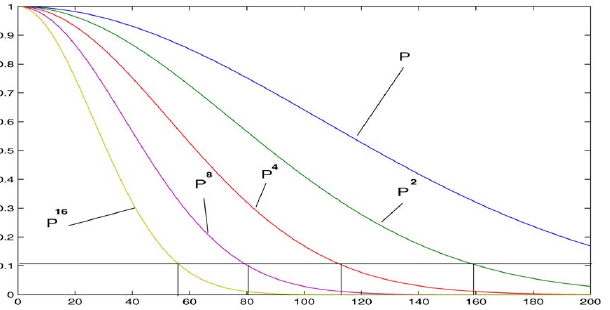
\includegraphics[width=0.72\linewidth]{paper_figures/P03_F03_page08.png}
\caption{Cropped figure panel containing the P03 Figure 3 spectrum plot discussed
as derived low-pass evidence.  Reproduced from Coifman and Lafon (2006),
Figure 3, PDF p. 12, from the canonical reading copy, for internal review
only.}
\end{figure}

\subsection{P04: Variable Bandwidth Diffusion Kernels}

\citet{berry2016variable} ask what changes when the diffusion kernel bandwidth
is local:
\[
  K_\epsilon^S(x,y)
  =
  h\!\left(
    \frac{\|x-y\|^2}{\epsilon\rho(x)\rho(y)}
  \right).
\]
The paper's practical Gaussian version uses
\[
  K_\epsilon^S(x_i,x_j)
  =
  \exp\left(
    -\frac{\|x_i-x_j\|^2}
          {4\epsilon\rho(x_i)\rho(x_j)}
  \right).
\]
The bandwidth \(\rho\) is often taken as \(q^\beta\), where \(q\) is sampling
density.  The limiting operator has the form
\[
  L_{\alpha,\rho}f
  =
  \Delta f
  +2(1-\alpha)\frac{\nabla f\cdot\nabla q}{q}
  +(d+2)\frac{\nabla f\cdot\nabla\rho}{\rho}.
\]
When \(\rho=q^\beta\), this becomes
\[
  L_{\alpha,\beta}f
  =
  \Delta f+
  c_1\frac{\nabla f\cdot\nabla q}{q},
  \qquad
  c_1=2-2\alpha+d\beta+2\beta.
\]
The audit notes that sign conventions for \(\Delta\) must be stated when
comparing this formula to graph smoothing or heat semigroups.

P04 is important for SIMODS because it shows that local scale is not just a
numerical patch.  It changes the continuum operator unless the normalization
parameters are chosen deliberately.  It supports variable-bandwidth
kernel-conductance comparators and density-correction diagnostics.  It does
not describe the current \code{fit.rdgraph.regression()} overlap-density
operator.

\subsection{P05: Gaussian Fields and Harmonic Functions}

\citet{zhu2003semisupervised} treat graph weights as the basis for
semi-supervised interpolation.  Given labeled and unlabeled vertices, the
harmonic solution minimizes graph energy subject to labeled boundary values,
leading to a Laplacian block system.  The weights are similarities/affinities,
and in the electrical-network interpretation they may be read as conductances.
Outside that interpretation, the safer phrase is ``weight/affinity,
interpretable as conductance.''

The paper connects harmonic functions, Gaussian random fields, graph cuts, and
kernel classifiers.  The relevant SIMODS lesson is direct: changing the edge
weights changes the interpolation.  If labels or feature values are graph
signals, the graph weights define what it means for the prediction to vary
smoothly away from observed values.

The audit corrected two convention points.  First, the heat-kernel sign should
be written as \(K_t=e^{-t\Delta}\) under the paper's convention.  Second, the
Rayleigh quotient numerator uses an unhalved double sum; the standard
symmetric-Laplacian energy includes a \(1/2\) factor.

\subsection{P06: Manifold Regularization}

\citet{belkin2006manifold} develop a learning framework with an ambient
regularizer and an intrinsic regularizer.  The graph Laplacian term is the
finite-sample proxy for intrinsic manifold regularity.  In the graph form,
large weights penalize variation between neighboring examples, so the
conductance/affinity choice controls which functions are preferred.

For SIMODS, P06 supports a regularization interpretation of graph smoothing.
The same operator that defines low-pass filtering can also be viewed as a
penalty in a learning objective.  This is useful for explaining why GCV over
graph smoothers is a non-oracle graph-selection candidate: a good graph should
make relevant signals predictable or low energy without relying on oracle
embedding metrics.

The audit emphasized precision around factor conventions and experimental
weight details.  The paper's Eq. (4) prints an unhalved double sum as
\(f^\top Lf\); this should be normalized carefully in synthesis.  The WebKB
description says weights are based on cosine distances, but the exact affinity
transform is not specified in the PDF.  Therefore it should not be turned into
a precise implementation recipe.

\subsection{P07: Graph Signal Processing}

\citet{shuman2013emerging} is the core source for graph-spectral smoothing
semantics.  A graph Fourier basis comes from Laplacian eigenvectors:
\[
  L\chi_\ell=\lambda_\ell\chi_\ell.
\]
The graph Fourier transform expands a signal in this basis, and a graph filter
multiplies each coefficient by a response \(h(\lambda_\ell)\):
\[
  \hat f_{\mathrm{filtered}}
  =
  \sum_\ell h(\lambda_\ell)\hat f(\lambda_\ell)\chi_\ell.
\]
This is exactly the language SIMODS needs when describing low-pass graph
smoothing.  The graph, weights, Laplacian normalization, and \(h(\lambda)\)
together define the smoother.

P07 should be cited primarily for graph-spectral smoothing, not for a
particular graph-construction recipe.  It also gives a valuable warning:
individual eigenvectors inside repeated or nearly repeated eigenspaces are not
unique; the meaningful object is the eigenspace or filter action.  Comparator
discussions should always name the actual spectral response \(h(\lambda)\),
such as heat, Tikhonov, polynomial, or idealized low-pass.

\subsection{P08: Graph Laplacian Convergence on Random Neighborhood Graphs}

\citet{hein2007graph} analyze convergence of graph Laplacians under random
geometric graph sampling, including unnormalized, random-walk, and normalized
operators.  The paper is a key warning against treating ``the graph
Laplacian'' as a single object.  Different normalizations converge to
different continuum operators and can place eigenfunction sign changes in
different density regions.

For conductance design, P08 matters because it separates graph support,
kernel weights, degree normalization, density effects, and limiting operator.
If a SIMODS comparator uses a heat kernel, inverse length, or self-tuned
kernel, the normalization choice remains a scientific choice.  A density-aware
operator may be useful for cluster assumptions; a density-invariant operator
may be better for geometric recovery.

The audit resolved the mapping to \code{gflow}: the current
\code{fit.rdgraph.regression()} operator is a custom mass-symmetrized spectral
smoother using overlap-density/Riemannian-complex conductance.  It is not
directly P08's random-walk, unnormalized, or symmetric-normalized Laplacian.
The audit also notes that \(k(0)=0\) removes self-loops and compact support is
part of the main non-compact consistency setup.

\subsection{P09: Theoretical Foundation for Laplacian-Based Manifold Methods}

\citet{belkin2008towards} provide theoretical support for the idea that graph
Laplacians built from local kernels can approximate manifold differential
operators.  The paper is a baseline for heat-kernel and Laplace-Beltrami
interpretations of graph smoothness.  Its role in SIMODS should be theoretical
framing: it does not guarantee finite-sample performance for arbitrary
biological graphs or for the current \code{gflow} overlap-density operator.

The post-audit notes are important.  The final synthesis must state the
paper's Laplacian sign convention before comparing equations to heat smoothing
or graph-signal filtering.  It must also preserve the distinction between
theorem settings involving \(\vol(M)\) and density scaling.  Coifman-Lafon
\(\alpha\)-normalization can be mentioned contextually here, but detailed
\(\alpha\) claims should be sourced to P03/P04.

P09 supports the practical reporting rule that any SIMODS kernel-conductance
smoother should document four ingredients: distance, bandwidth rule,
degree/density normalization, and target operator or practical surrogate.

\subsection{P10: kNN Self-Tuned Kernel Graph Laplacian Convergence}

\citet{cheng2022knn} connect self-tuned kernels to graph Laplacian convergence
with kNN-derived local scales.  This is the most direct theory source for the
relationship between nearest-neighbor scale estimation and adaptive
kernel-conductance rules.  The paper separates Dirichlet-form convergence from
pointwise operator convergence, a distinction that matters for smoothing:
penalty-based smoothers align more naturally with Dirichlet-form statements,
whereas pointwise Laplacian estimation needs stronger assumptions.

For SIMODS, P10 supports a planned comparator of the form
\[
  c_{ij}
  =
  \exp\!\left(
    -\frac{\ell_{ij}^2}{\widehat\rho_i\widehat\rho_j}
  \right)
\]
or the paper's more precise kNN self-tuned scaling.  However, kNN bandwidth
estimation and graph support construction are different design choices.  A
SIMODS implementation must decide whether local scales are estimated from all
point-cloud neighbors, graph-neighbor edge lengths, or another structure.

The audit also cautions that special \(\alpha\) choices are operator-specific.
Do not transfer a default from diffusion maps or variable-bandwidth kernels
without restating the exact construction.  The MNIST/outlier result should be
treated as secondary empirical evidence, not convergence proof.

\section{Synthesis by Task}

\subsection{Embedding and Manifold Learning}

P02, P03, P04, P08, P09, and P10 all contribute to manifold-learning
interpretations, but they emphasize different levels of the pipeline.  P02
introduces the graph construction plus generalized eigenproblem.  P09 supplies
theoretical foundation for local kernel graph Laplacians.  P03 adds Markov
diffusion and density normalization.  P04 and P10 introduce adaptive local
scale and show that local bandwidth changes the limiting operator.  P08 warns
that normalization and density are not cosmetic.

For SIMODS, this means a graph-smoothing benchmark should not report only
``heat kernel'' or ``self-tuned kernel.''  It should report graph support,
kernel formula, bandwidth/local-scale rule, degree normalization, and filter
response.

\subsection{Spectral Clustering}

P01 uses local-scale Gaussian affinities to reduce global bandwidth fragility
in spectral clustering.  P08 gives theoretical background on how graph
normalization affects clustering-related eigenfunctions.  P02 links
Laplacian eigenmaps to spectral clustering through the same graph smoothness
objective.  These papers support self-tuned and density-aware comparator
families, but they do not directly provide a GCV graph-selection criterion.

\subsection{Diffusion Geometry}

P03 and P04 are the main diffusion-geometry sources.  They make clear that
kernel weights are only the first stage.  After degree and density
normalization, the operator may be a Markov transition matrix, an infinitesimal
generator, or a symmetric conjugate.  Diffusion powers \(P^t\) and heat
semigroups \(e^{-tL}\) are low-pass smoothers with different normalizations.

\subsection{Semi-Supervised Learning and Graph Regression}

P05 and P06 support the learning/regression view.  P05 solves harmonic
interpolation on a weighted graph.  P06 uses graph Laplacian regularization in
a broader learning objective.  For SIMODS GCV, these papers justify measuring
how well a graph supports smooth prediction of feature signals.  They also warn
that if the feature task is outcome-specific, the selector may become
task-aligned rather than geometry-general.

\subsection{Graph Signal Processing and Smoothing}

P07 is the clearest conceptual home for low-pass smoothing.  It says that the
same graph signal can be smooth on one graph and rough on another, because
smoothness is defined by the graph operator.  This is the logic behind
non-oracle graph selection by feature-signal GCV: candidate graphs are scored
by whether meaningful signals are low-frequency and predictable.  P07 also
forces reporting of \(h(\lambda)\), not just the graph.

\section{Synthesis by Conductance Family}

\begin{longtable}{p{0.22\linewidth}p{0.23\linewidth}p{0.22\linewidth}p{0.23\linewidth}}
\caption{Conductance/kernel families and synthesis role.}\\
\toprule
Family & Formula & Main sources & SIMODS interpretation\\
\midrule
\endhead
Inverse length &
\((\ell+\epsilon)^{-\alpha}\) &
contextual comparator; not a reviewed paper's central formula &
Best direct metric-geometry smoother comparator.\\
Heat/RBF &
\(\exp(-\ell^2/t)\), \(\exp(-\ell^2/(4t))\) &
P02, P03, P09 &
Natural for point-cloud diffusion and Laplace-Beltrami approximation.\\
Exponential/Laplace &
\(\exp(-\ell/\sigma)\) &
H005 requested family; less central in Tier 1 corpus &
Useful robustness comparator, but needs additional source support.\\
Self-tuned Gaussian &
\(\exp[-\ell_{ij}^2/(\sigma_i\sigma_j)]\) &
P01, P10 &
Local-scale comparator for nonuniform sampling.\\
Variable bandwidth &
\(h(\ell^2/[\epsilon\rho_i\rho_j])\) &
P04, P10 &
Theory-backed adaptive bandwidth; operator changes with \(\rho\) and normalization.\\
Density-normalized &
\(k/(q_i^\alpha q_j^\alpha)\) &
P03, P04, P08 &
Separates geometry from sampling density when desired.\\
Binary support &
\(c_{ij}=1\) on graph edges &
P02, P08 &
Control comparator isolating graph support from metric weights.\\
\bottomrule
\end{longtable}

\subsection{Why Not Always Use Inverse Length?}

Inverse length is attractive because it respects a direct resistance intuition:
short edges should transmit signal strongly; long edges should transmit weakly.
For SIMODS, this is exactly why it should be a planned comparator.  But the
reviewed literature shows why researchers often use other forms:

\begin{itemize}
  \item Heat kernels approximate local diffusion and suppress long edges
    exponentially rather than algebraically.
  \item Gaussian bandwidths provide a scale parameter that defines locality.
  \item Self-tuned kernels adjust that scale under nonuniform sampling.
  \item Density normalization can remove sampling-density bias from the
    limiting operator.
  \item Markov normalization turns affinities into transition probabilities
    and makes diffusion distances path-based rather than edge-local.
  \item Graph signal filters separate graph construction from the spectral
    response applied to the signal.
\end{itemize}

Thus inverse length is one scientifically meaningful choice, not the universal
default.

\section{Theory Results and Their Benchmark Implications}

\begin{longtable}{p{0.12\linewidth}p{0.22\linewidth}p{0.22\linewidth}p{0.33\linewidth}}
\caption{Theory themes relevant to SIMODS comparator design.}\\
\toprule
Source & Setting & Operator issue & Implication\\
\midrule
\endhead
P02 & Local graph on point samples & Heat weights and generalized eigenproblem & Heat-kernel weights are principled but bandwidth and graph support remain choices.\\
P03 & Diffusion maps & \(\alpha\)-normalization and Markov powers & Degree/density normalization changes the geometry; \(P^t\) is a low-pass diffusion smoother.\\
P04 & Variable bandwidth diffusion & \(\rho=q^\beta\), \(\alpha\), dimension \(d\) & Local scale can stabilize sparse regions but changes drift terms unless normalized deliberately.\\
P08 & Random neighborhood graph convergence & Unnormalized/random-walk/normalized limits & Normalization can move eigenfunctions and density effects; do not claim one generic Laplacian target.\\
P09 & Laplacian-based manifold methods & Kernel graph Laplacian to manifold operator & Kernel-distance smoothers need documented distance, bandwidth, normalization, and target operator.\\
P10 & kNN self-tuned kernels & Local kNN scale and convergence & kNN bandwidth estimation is a serious theory-backed local-scale comparator, especially for Dirichlet-form smoothing.\\
\bottomrule
\end{longtable}

\section{Implications for gflow and SIMODS}

\subsection{Recommended Comparator Families}

The future non-oracle graph-selection benchmark should compare at least:
\begin{align}
  c_e^\rho &= \frac{1}{\max(\rho_1(e),10^{-10})}
  &&\text{current \code{fit.rdgraph.regression()} semantics},\\
  c_e^{\mathrm{len}} &= \frac{1}{\ell_e+\epsilon}
  &&\text{direct metric-length conductance},\\
  c_e^{\mathrm{rbf}} &= \exp(-\ell_e^2/\sigma^2)
  &&\text{heat/RBF conductance},\\
  c_e^{\mathrm{exp}} &= \exp(-\ell_e/\sigma)
  &&\text{exponential-distance conductance},\\
  c_{ij}^{\mathrm{self}} &=
    \exp\!\left(-\frac{\ell_{ij}^2}{\sigma_i\sigma_j}\right)
  &&\text{self-tuned local-scale conductance}.
\end{align}
For diffusion-style variants, the benchmark must state whether the smoother is
formed from a symmetric Laplacian, a random-walk matrix \(P\), a symmetric
Markov conjugate, or another mass-symmetrized operator.

\subsection{Recommended Diagnostics}

The benchmark should not rely on GCV alone.  It should record:
\begin{itemize}
  \item selected graph parameter and selected smoothing parameter;
  \item GCV score and effective degrees of freedom;
  \item transfer function \(h(\lambda)\);
  \item eigenvalue spectrum and spectral gaps;
  \item eigenfunction localization or sign-change diagnostics;
  \item clean-function RMSE on synthetic known signals;
  \item agreement with oracle geodesic-isometry performance on synthetic quad
    benchmarks;
  \item sensitivity to sampling density and noise.
\end{itemize}

\subsection{How to Phrase Claims in the Manuscript}

The manuscript can safely say:

\begin{itemize}
  \item Graph smoothing is operator-dependent: the graph support, edge weights,
    normalization, and spectral response define what ``low frequency'' means.
  \item Heat/RBF, self-tuned, and density-normalized kernels are standard
    families for graph Laplacians and diffusion operators.
  \item Local-scale kernels are motivated by nonuniform sampling and can change
    both numerical behavior and continuum limits.
  \item The current \code{gflow} smoother is an overlap-density /
    Riemannian-complex smoother, not a direct length-kernel smoother.
  \item A controlled SIMODS benchmark should test whether current
    overlap-density smoothing and length/kernel-conductance smoothing select
    graph parameters that agree with oracle geodesic-isometry performance.
\end{itemize}

The manuscript should avoid saying:

\begin{itemize}
  \item that \code{fit.rdgraph.regression()} currently implements
    \(1/(\ell+\epsilon)\), Gaussian, or self-tuned conductances;
  \item that self-tuned bandwidth estimation is the same as cKNN graph support;
  \item that one \(\alpha\) or Laplacian normalization has the same meaning
    across all reviewed papers;
  \item that asymptotic manifold theory guarantees finite-sample SIMODS
    performance without a matching benchmark.
\end{itemize}

\section{Evidence Label Table}

\begin{longtable}{p{0.26\linewidth}p{0.12\linewidth}p{0.27\linewidth}p{0.25\linewidth}}
\caption{Selected synthesis claims with evidence labels.}\\
\toprule
Claim & Label & Source & Notes\\
\midrule
\endhead
Self-tuned spectral clustering uses \(\exp[-d^2/(\sigma_i\sigma_j)]\). &
explicit & P01, Eq. (1) & Local scale from \(K\)th neighbor distance.\\
Laplacian Eigenmaps use heat weights and \(Ly=\lambda Dy\). &
explicit & P02 & Heat bandwidth conventions \(t\) and \(4t\) both appear.\\
Diffusion maps define diffusion distance through \(P^t\) spectra. &
explicit & P03 & Markov normalization central.\\
Increasing diffusion time damps smaller Markov eigenvalues. &
derived & P03 Figure 3 and formulas & Low-pass language is synthesis.\\
Variable bandwidth kernels change continuum drift terms. &
explicit & P04 & Depends on \(\alpha,\beta,d\).\\
Harmonic graph interpolation depends on edge weights. &
derived & P05 & Weight-as-conductance language safest in electrical interpretation.\\
Graph filters require reporting \(h(\lambda)\). &
derived/contextual & P07 & Essential for SIMODS comparator reporting.\\
Normalization changes graph Laplacian limits and eigenfunctions. &
explicit/derived & P08 & Avoid generic ``the graph Laplacian.''\\
Kernel graph Laplacian theory supports planned heat-kernel comparators. &
derived & P09 & Applicability depends on assumptions.\\
kNN self-tuned kernels support adaptive local-scale comparators. &
derived & P10 & Distinguish bandwidth estimation from support construction.\\
Current \code{gflow} smoother is overlap-density, not length/RBF/self-tuned. &
contextual & H003/H004 source audit plus H005 scope & Not a claim from the reviewed papers.\\
\bottomrule
\end{longtable}

\section{Open Risks and Questions}

\begin{enumerate}
  \item The Tier 1 corpus is strong for heat/RBF, diffusion, self-tuned, local
    bandwidth, and graph signal filtering.  It is weaker for direct
    inverse-length and \(\exp(-\ell/\sigma)\) conductance rules as primary
    literature topics.  Those may need Tier 2 additions if the final
    manuscript foregrounds them.
  \item Several sources use different Laplacian sign conventions.  Final
    equations should state whether \(L\) is positive semidefinite and whether
    heat is \(e^{-tL}\) or \(e^{t\Delta}\) under a PDE sign convention.
  \item Local bandwidth and graph support are separate implementation choices.
    A SIMODS self-tuned comparator should define both.
  \item If SVG explanatory figures are used in a \code{pdflatex} report, they
    should be rendered to PDF or PNG.
  \item Reproduced paper-figure cropped figure panels are now stored under
    \code{paper\_figures/} and tracked by
    \code{paper\_figure\_screenshots.yml}.  These are internal-review
    screenshots from canonical reading copies; if the final public supplement
    uses paper figures, permissions and reproduction labels will still be
    needed.
\end{enumerate}

\section{Conclusion}

The literature supports a principled benchmark in which the current
overlap-density/Riemannian-complex \code{gflow} smoother is compared against
direct length and kernel conductance smoothers.  The most important design
lesson is that the conductance rule cannot be separated from graph support,
normalization, spectral response, and task.  Heat kernels emphasize local
diffusion; self-tuned kernels adapt to local sampling scale; variable-bandwidth
and density-normalized kernels change continuum limits; graph signal processing
turns the resulting operator into a filter \(h(\lambda)\).  A SIMODS
non-oracle graph-selection criterion should therefore report the full operator
construction and should judge candidate smoothers by agreement with oracle
geodesic-isometry performance, signal reconstruction behavior, and robustness
diagnostics rather than by GCV alone.

\appendix
\section{Local Artifact Inventory}

The H005 workspace contains:
\begin{itemize}
  \item \code{source\_manifest.yml}: source acquisition manifest.
  \item \code{references.bib}: BibTeX database for this report.
  \item \code{paper\_memos/P*.md}: revised-after-audit paper review memos.
  \item \code{audits/P*\_audit.md}: paper-specific audit memos.
  \item \code{sources/pdf/P*.pdf}: cached canonical Tier 1 reading copies.
  \item \code{figures/P01\_self\_tuned\_kernel\_toy.png},
    \code{figures/P04\_local\_bandwidth\_conductance\_curve.png},
    \code{figures/P05\_three\_node\_harmonic\_interpolation.svg},
    \code{figures/P07\_graph\_filter\_pipeline.png}, and
    \code{figures/P09\_operator\_limit\_map.svg}: original internal
    explanatory figures created by reviewers.
\end{itemize}

\bibliographystyle{plainnat}
\bibliography{references}

\end{document}
